\documentclass[11pt]{article}
\usepackage[margin=1in]{geometry}
\usepackage{amsmath,amssymb,booktabs,array,microtype,enumitem,xcolor,graphicx,hyperref}
\hypersetup{colorlinks=true,linkcolor=blue!55!black,citecolor=blue!55!black,urlcolor=blue!55!black}
\newcommand{\jev}{\textsc{Jev}}

\title{\textbf{Decisions, Not Tokens}\\\large A Survey of Typed, Calibrated, and Machine-Native Decision Models from Classical Classifiers to Jev}
\author{Anonymous Authors}
\date{Full working draft --- 21 September 2026}

\begin{document}
\maketitle

\begin{abstract}
Large language models have made natural language a general computing interface, but many software components need only a judgment, a bounded choice, or a score that triggers an action. Moving open-ended text into a control flow usually adds parsing, validation, review, and authorization layers. In September 2026, TypeSafe AI introduced \emph{System One Models} under its ``Machine-Native Intelligence'' thesis and released Jev as the first public instance: given state and typed questions, it returns Choice, Score, or Noul values with probabilities \cite{typesafe2026home,almeida2026jev,typesafe2026systemone,typesafe2026docs}. The launch materials report end-to-end latency of 70--500 ms and a price of USD 0.042 per million input tokens; both are first-party claims awaiting independent replication \cite{almeida2026jev}. This survey uses \emph{machine-native decision model} as an umbrella analytical term that connects this industrial category to structured prediction, constrained decoding, probability calibration, selective prediction, learning to defer, decision-focused learning, and multi-model routing. We define the object operationally as a model that maps state and a predeclared decision specification to a software-consumable typed value or distribution, with uncertainty connected to execution, verification, routing, abstention, or escalation. We organize the literature along five dimensions and develop an evaluation framework spanning structural validity, semantic correctness, probabilistic reliability, selective risk, latency, cost, and distribution shift. Type constraints remove a class of interface failures, calibration gives probabilities a population-level interpretation, and selective policies make uncertainty operational; dependable automation requires all three to be evaluated with task loss, changing distributions, action costs, and workflow outcomes.
\end{abstract}

\section{Introduction}

Large language models have brought content generation into search, customer support, code execution, and agent workflows. Many production steps, however, do not require a human-facing response. A support system may need to route ``my card was charged twice'' to billing, technical, or account; an agent controller may need to continue, review, or stop a tool call; and a risk system may need a score that triggers blocking or human escalation. Open-ended generation can supply more information than these tasks require while leaving format parsing, factual verification, and authorization to downstream components. Production stacks therefore often add JSON parsing, retries, rule-based validators, LLM-as-a-judge checks, stronger-model review, and human fallback. Each component can reduce a particular failure mode while accumulating latency, cost, and additional error surfaces.

TypeSafe frames this interface mismatch as one between human-facing strings and software-facing decisions. Under the label ``Machine-Native Intelligence,'' the company introduced System One Models as a class of models for fast, structured decisions inside software; Jev is its first public instance \cite{typesafe2026home,almeida2026jev,typesafe2026systemone}. In TypeSafe's refund example, customer text, transactions, and policy form the state; the model evaluates whether a refund was requested, whether evidence indicates a duplicate charge, and whether policy supports the refund; code then combines the answers and routes the case to action or review \cite{typesafe2026systemone}. Jev exposes Choice, Score, and Noul primitives over predeclared answer spaces. First-party materials report parallel evaluation, 70--500 ms end-to-end latency, USD 0.042 per million input tokens, and 40--200-fold speedups on selected workflows \cite{typesafe2026docs,almeida2026jev}. The vendor also states that these gains likely represent the high end of real-world improvements and that its workflow references are generated by strong external models. The figures are therefore testable hypotheses rather than independent evidence.

The System One label is new, whereas its component problems have long research histories. Classifiers and structured predictors produce bounded labels or joint structures; constrained decoding enforces grammars and schemas; calibration connects confidence to empirical frequencies; selective prediction and learning to defer govern automation; and decision-focused learning and routing incorporate action costs and compute budgets. The scale of recent benchmarks illustrates why these properties need separate measurement: JSONSchemaBench tests constrained decoding against 10,000 real-world schemas \cite{geng2025jsonschema}, while a unified routing study covering more than 400,000 instances, 21 datasets, and 33 models finds that sophisticated routers do not consistently dominate simple baselines under a common protocol \cite{li2026routerbench}. Together, these lines separate four objectives that a production workflow must reconnect: structural validity, semantic correctness, probabilistic reliability, and decision utility.

This survey follows TypeSafe's machine-native intelligence and System One framing and uses \emph{machine-native decision model} as an umbrella analytical term. The origin of the industrial thesis and category belongs to TypeSafe; our contribution is to delimit the concept, locate it within the prior literature, and make its claims measurable. We ask how typed probabilistic interfaces relate to classifiers, structured generators, reward models, routers, and agents; how accuracy, calibration, selective risk, and utility should be measured together; what Jev's public evidence establishes; and which reproducible benchmarks the field now needs.

Our contributions are fourfold. We clarify the provenance and operational boundary of machine-native decision models; synthesize the literature through a five-dimensional taxonomy; separate structural validity, semantic correctness, probabilistic reliability, and decision utility; and audit Jev's evidence by distinguishing documented facts, vendor reports, independent evidence, and unresolved questions.

\begin{figure*}[t]
\centering
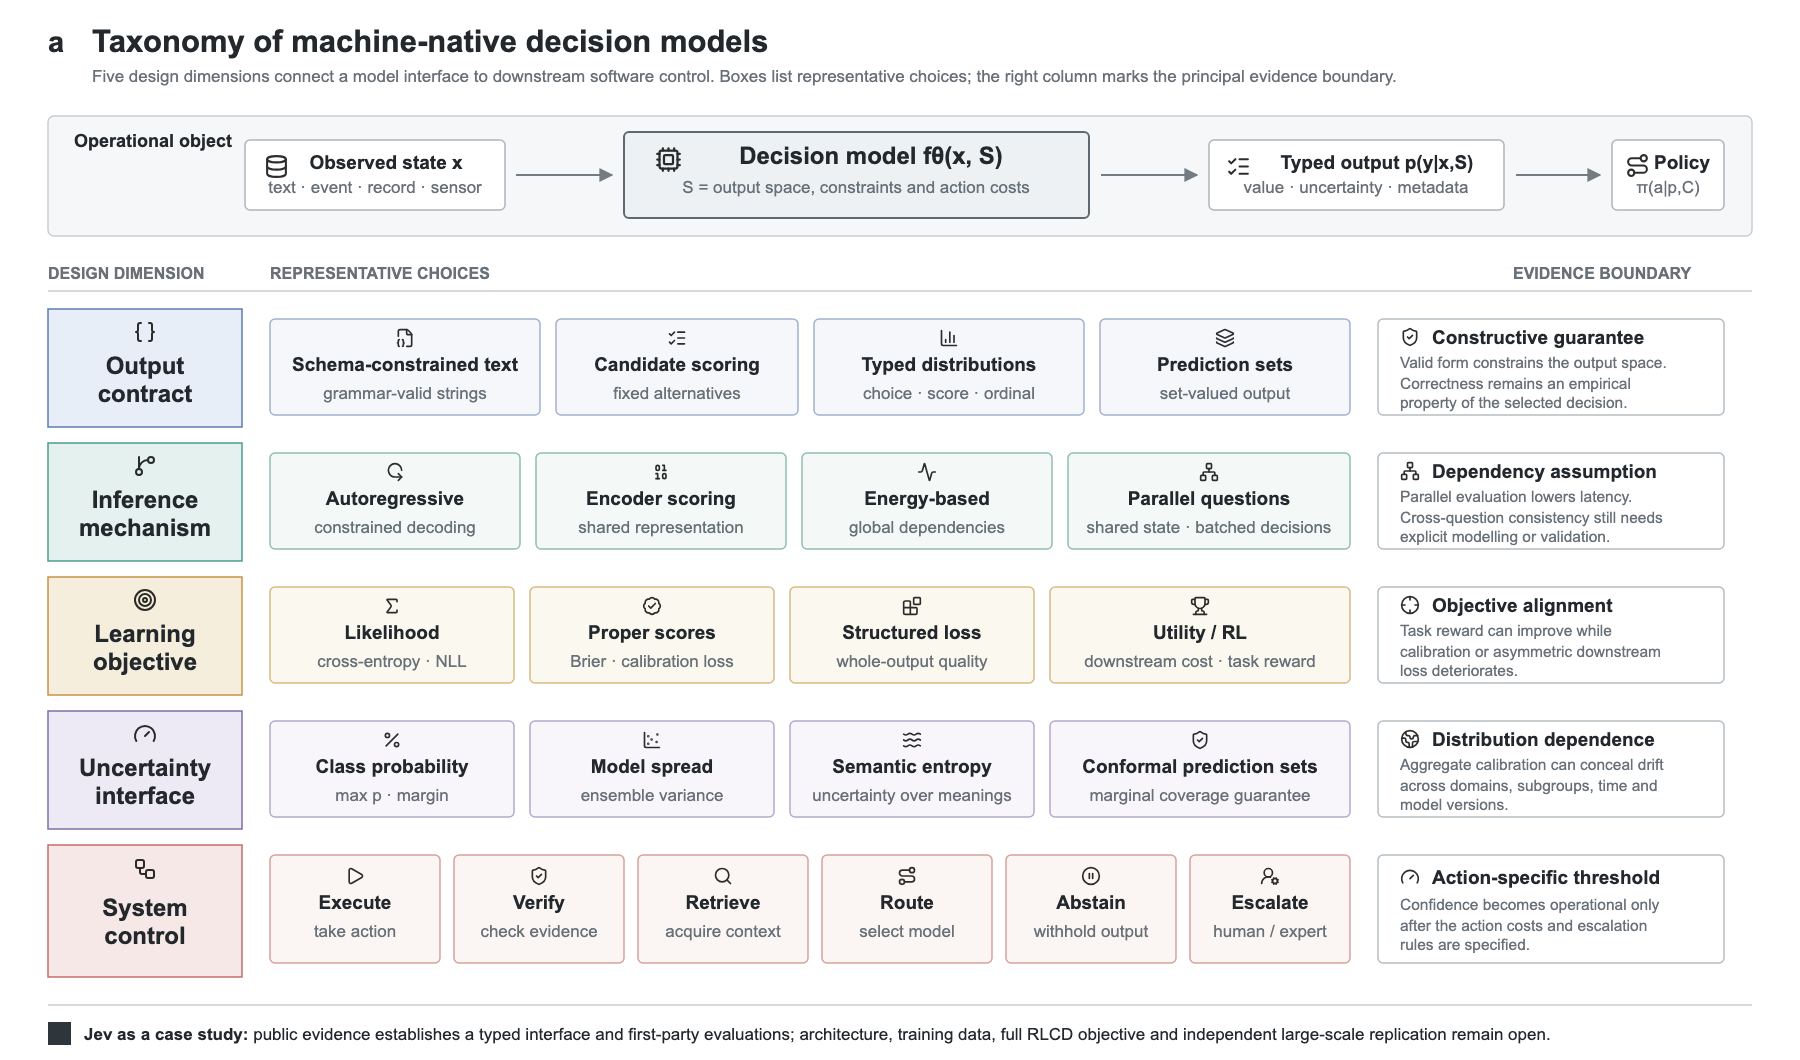
\includegraphics[width=\textwidth]{figures/fig1_machine_native_landscape.png}
\caption{\textbf{Taxonomy of machine-native decision models.} Output contract, inference mechanism, learning objective, uncertainty interface, and system control jointly determine what a model may return, how its confidence should be interpreted, and which downstream action software should take. The right column states the principal evidence boundary for each design dimension. Jev is treated as a contemporary case whose public evidence currently establishes an interface more clearly than a reproducible architecture.}
\label{fig:landscape}
\end{figure*}

\section{Scope, Definition, and Review Method}

\subsection{Concept provenance and operational definition}

The immediate provenance of this concept is TypeSafe's positioning of Jev. Its website uses ``Machine-Native Intelligence'' for the broader direction, while the launch article and documentation explicitly introduce ``System One Models'' as a class of models that return fast, typed decisions and probabilities for software \cite{typesafe2026home,almeida2026jev,typesafe2026systemone}. We use \emph{machine-native decision model} as an umbrella analytical term that places this industrial thesis within the historical lineages of discriminative models, structured prediction, constrained generation, probabilistic prediction, and routing. The category-level thesis is attributed to TypeSafe; this survey contributes a unified scope, formal object, five-dimensional taxonomy, and four-layer evaluation framework.

Let $x$ denote observed state and $S=(\mathcal{Y},\tau,C)$ a decision specification, where $\mathcal{Y}$ is the output space, $\tau$ contains type or structural constraints, and $C(a,y,x)$ is the cost of action $a$ when the outcome is $y$. A machine-native decision model returns
\begin{equation}
 f_\theta(x,S)=\bigl(\hat p(y\mid x,S),m\bigr),
\end{equation}
where $\hat p$ is a distribution over finite candidates, ordinal values, or constrained objects and $m$ is optional metadata. A policy $\pi$ maps the result to execution, checking, tool use, model routing, abstention, or human escalation.

Three properties make the definition operational. The decision space is declarable before inference; software can parse the result deterministically; and an uncertainty or abstention signal participates in downstream control. The definition concerns an interface and control loop, so an encoder, energy model, or constrained autoregressive model can implement it. Free text followed by a regular expression is a weak implementation. A typed output without a reliability assessment or action policy remains insufficient for consequential automation.

\subsection{Four evaluation layers}

Table~\ref{tab:layers} separates four properties that benchmarks often blend. Structural validity says that an object parses. Semantic correctness concerns the task label or verifiable outcome. Calibration relates stated probability to empirical frequency over sets of examples. Decision utility evaluates the consequences of acting. A claim of ``zero hallucinations'' limited to schema matching supports the first layer only. Global calibration can coexist with severe miscalibration in a domain, subgroup, action class, or later time period \cite{silvafilho2023calibration}.

\begin{table}[t]
\centering\small
\begin{tabular}{p{.19\linewidth}p{.28\linewidth}p{.23\linewidth}p{.21\linewidth}}
\toprule
Layer & Question & Measures & Counterexample \\
\midrule
Structural validity & Does the output satisfy its schema and type? & Parse and schema-valid rates & Valid JSON names the wrong account \\
Semantic correctness & Does the decision match the label or fact? & Accuracy, F1, task loss & Complete probability object, wrong choice \\
Probabilistic reliability & Do $q$-confidence events occur about $q$ of the time? & NLL, Brier, ECE, reliability plots & A 90\% bin is correct 65\% \\
Decision utility & What follows after the system acts? & Expected utility, selective risk, action cost & High accuracy, costly false execution \\
\bottomrule
\end{tabular}
\caption{Four evaluation layers for machine-native decisions.}
\label{tab:layers}
\end{table}

\subsection{Evidence policy}

We searched ACL Anthology, PMLR, NeurIPS proceedings, OpenReview, arXiv, Crossref, official documentation, and public code using combinations of \emph{calibration}, \emph{selective prediction}, \emph{abstention}, \emph{learning to defer}, \emph{structured prediction}, \emph{constrained decoding}, \emph{decision-focused learning}, \emph{LLM routing}, and \emph{Jev}. Peer-reviewed work supports general technical claims; preprints indicate fast-moving directions; vendor sources support public interfaces and self-reported results. The search cutoff is 21 September 2026.

\section{Technical Lineages: From Prediction to Action}

\subsection{Classification, structured prediction, and type contracts}

Classical classifiers produce finite labels or categorical distributions and are already machine-readable, although independent labels can flatten a structured action. Structured prediction represents dependencies among output variables. Structured Prediction Energy Networks score entire structured outputs with a learned energy function \cite{belanger2016spen}. Calibration of structured NLP predictors further shows that sequence-level confidence must account for label dependencies and differs from calibrating independent tokens \cite{jagannatha2020structured}.

Constrained generation reaches typed outputs from the opposite direction: it retains an autoregressive language model while masking tokens that violate a grammar or schema. PICARD incrementally rejects invalid tokens for text-to-SQL \cite{scholak2021picard}. Grammar-constrained decoding extends formal and input-dependent grammars to extraction, entity disambiguation, and parsing \cite{geng2023grammar}. JSONSchemaBench evaluates open-source libraries and commercial APIs on 10,000 real-world schemas, separating schema coverage, efficiency, and generation quality \cite{geng2025jsonschema}. Syntax is thus an independently measurable capability. Semantic quality should be compared with and without constraints because a grammar can force a low-probability valid continuation.

\subsection{Probability calibration}

A predictor is calibrated when examples receiving confidence near $q$ are correct with frequency near $q$, under a stated distribution and grouping. Modern neural networks often produce overconfident errors, and temperature scaling remains a strong post-hoc baseline \cite{guo2017calibration}. Pretrained Transformers were better calibrated than earlier neural baselines on several in-domain text-classification tasks, while calibration still degraded out of domain \cite{desai2020calibration}. Question-answering work likewise finds that token probabilities, verbalized confidence, and answer correctness do not coincide automatically \cite{jiang2021know,lin2022verbalized}.

Large models can sometimes estimate whether an answer is true or whether they know it, with improved performance at larger scales, although cross-task calibration remains limited \cite{kadavath2022know}. Open-ended generation adds another complication: different strings can carry the same meaning. Semantic entropy clusters answers by meaning before estimating uncertainty and improves error detection on several question-answering tasks \cite{kuhn2024semantic}. The uncertainty representation must match the event on which software acts, and deployment calibration requires target-domain data.

\subsection{Selective prediction and learning to defer}

Selective prediction introduces a selection function $g(x)$ and answers only when $g(x)=1$. Coverage is $\phi=\mathbb{E}[g(x)]$, and selective risk is
\begin{equation}
R_{\mathrm{sel}}=\frac{\mathbb{E}[\ell(f(x),y)g(x)]}{\mathbb{E}[g(x)]}.
\end{equation}
Varying a confidence threshold traces a risk--coverage curve. SelectiveNet jointly learns prediction and rejection at a target coverage \cite{geifman2019selectivenet}. NLP evaluations show that a confidence ranking that works in domain can fail to isolate errors under distribution shift \cite{gu2023selective,varshney2022selective}. Thresholds should therefore be selected from target risk, desired coverage, error costs, and a held-out calibration set.

Learning to defer incorporates an external decision maker into the objective. Early work jointly learned a prediction and PASS action while modeling the accuracy and bias of a downstream human \cite{madras2018defer}. Post-hoc approaches compare the base model's estimated error probability with expert cost, connecting human referral and adaptive model inference \cite{narasimhan2022defer}. The relevant unit is the team: a weaker standalone model can produce a better system when it identifies cases an expert handles well.

\subsection{Decision-focused learning}

Predictive loss and action value can diverge. A smaller demand-forecasting error may leave inventory cost unchanged if it occurs away from a decision boundary. Decision-focused learning differentiates through or approximates the downstream optimization problem so that the predictive component improves the decisions it induces \cite{wilder2019decision,mandi2023dfl}. A probability becomes actionable only after combination with available actions and costs. Robust evaluation should vary cost assumptions and guard against overfitting to a historical solver or policy.

\subsection{Routing, cascades, and dynamic computation}

Multi-model systems treat model selection as a decision. FrugalGPT learns cascades that trade API cost against quality \cite{chen2023frugalgpt}; RouteLLM learns to route between stronger and weaker models from preference data \cite{ong2024routellm}. Cascades call a cheap model first and escalate uncertain examples, saving cost at the price of tail latency. Pre-generation routers are faster but infer difficulty from the input alone. A 2026 benchmark spanning more than 400,000 instances, 21 datasets, and 33 models found that several sophisticated methods and commercial routers did not reliably beat simple baselines under a common protocol \cite{li2026routerbench}. Router results depend strongly on model portfolio, data split, cost schedule, and update frequency.

\section{Mathematical Foundations: From Confidence to Action}

\subsection{Typed probability interfaces}

For a decision with $K$ admissible alternatives, the model returns a point on the probability simplex,
\begin{equation}
\Delta^{K-1}=\left\{\mathbf p\in[0,1]^K:\sum_{k=1}^{K}p_k=1\right\},
\qquad \hat y=\arg\max_k p_k.
\end{equation}
The type system determines what the coordinates mean; the probabilistic model expresses relative belief among them. If a valid action may fall outside $\mathcal{Y}$, the contract should include an abstention symbol $\bot$ or an out-of-set event. Simplex validity alone can otherwise force a wrong closed-set decision.

\subsection{Calibration and strictly proper scores}

Let $c(X)=\max_k p_k(X)$ and let $\hat Y$ be the predicted class. Perfect confidence calibration requires
\begin{equation}
\Pr\!\left(Y=\hat Y\mid c(X)=q\right)=q,\qquad q\in[0,1].
\end{equation}
Finite-sample evaluation commonly partitions predictions into $M$ confidence bins $B_m$ and estimates
\begin{equation}
\operatorname{ECE}=\sum_{m=1}^{M}\frac{|B_m|}{n}
\left|\operatorname{acc}(B_m)-\operatorname{conf}(B_m)\right|.
\end{equation}
Because ECE depends on binning, it should be accompanied by strictly proper scores. The multiclass Brier score and negative log-likelihood are
\begin{align}
\operatorname{BS}&=\frac{1}{n}\sum_{i=1}^{n}\sum_{k=1}^{K}
\left(p_{ik}-\mathbb{1}[y_i=k]\right)^2,\\
\operatorname{NLL}&=-\frac{1}{n}\sum_{i=1}^{n}\log p_{i,y_i}.
\end{align}
Both use the full predictive distribution and penalize confident errors; NLL is especially sensitive when the true-class probability approaches zero. Accuracy remains necessary because a base-rate predictor may be reasonably calibrated while offering little discrimination.

\subsection{Selective risk, deferral, and costs}

A gate $g_\lambda(x)=\mathbb{1}[c(x)\geq\lambda]$ converts confidence into an automation policy. Its empirical coverage and selective risk are
\begin{equation}
\phi(\lambda)=\frac{1}{n}\sum_{i=1}^{n}g_\lambda(x_i),\qquad
R_{\mathrm{sel}}(\lambda)=
\frac{\sum_{i=1}^{n}\ell(f(x_i),y_i)g_\lambda(x_i)}
{\sum_{i=1}^{n}g_\lambda(x_i)}.
\end{equation}
The area under the resulting curve is $\operatorname{AURC}=\int_0^1R_{\mathrm{sel}}(\phi)\,d\phi$. Operational thresholds follow from costs. If correct automatic execution costs $C_{\mathrm{ok}}$, an error costs $C_{\mathrm{err}}$, and escalation costs $C_{\mathrm{esc}}$, execution under a calibrated binary correctness probability $p$ is preferred when
\begin{equation}
pC_{\mathrm{ok}}+(1-p)C_{\mathrm{err}}\leq C_{\mathrm{esc}}.
\end{equation}
This inequality makes a confidence threshold application-specific.

\subsection{Coverage guarantees and system objectives}

For a set-valued predictor $\Gamma_\alpha(X)$, conformal methods target finite-sample marginal coverage
\begin{equation}
\Pr\!\left(Y\in\Gamma_\alpha(X)\right)\geq 1-\alpha,
\end{equation}
under assumptions including exchangeability \cite{quach2024conformal}. A multi-model deployment can combine quality, cost, and latency as
\begin{equation}
\max_{\pi}\;\mathbb E[U(\pi(X),Y)]-\lambda\mathbb E[C_\pi(X)]-\mu\mathbb E[L_\pi(X)]
\quad\text{s.t.}\quad R_{\mathrm{sel}}\leq r_0.
\end{equation}
Here $\pi$ selects a model and a downstream action, $\lambda$ and $\mu$ encode resource preferences, and $r_0$ is a risk budget. This form turns claims of being more accurate, faster, or cheaper into an auditable Pareto trade-off.

\section{A Five-Dimensional Taxonomy}

\begin{table}[t]
\centering\small
\begin{tabular}{p{.17\linewidth}p{.25\linewidth}p{.27\linewidth}p{.22\linewidth}}
\toprule
Dimension & Representative values & Central question & Typical failure \\
\midrule
Output contract & Free text; constrained text; candidate scores; typed distributions & What can the model return? & Valid form, wrong meaning \\
Inference & Autoregressive; encoder; energy-based; parallel & How are alternatives and dependencies compared? & Inconsistent parallel answers \\
Learning objective & Likelihood; proper score; structured loss; utility; RL & Which behavior receives gradient or reward? & Accuracy--calibration trade-off \\
Uncertainty & Max probability; margin; ensemble; semantic entropy; set & What event does confidence describe? & Shift-induced miscalibration \\
System control & Execute; verify; route; abstain; escalate & What happens after prediction? & Unsafe threshold \\
\bottomrule
\end{tabular}
\caption{Taxonomy of machine-native decision models.}
\label{tab:taxonomy}
\end{table}

\paragraph{Output contract.} Contracts range from free text through schema-constrained text and candidate scoring to native typed distributions. The useful question is which errors become impossible by construction. An enumeration excludes unknown labels but may force a choice when the correct action is absent. An ordinal score encodes order while leaving adjacent levels ambiguous. Set-valued outputs preserve uncertainty but require a consumer that can handle several candidates.

\paragraph{Inference mechanism.} Autoregressive decoding offers flexible composition and cost proportional to output length. Encoders compare fixed candidates efficiently. Energy models express global dependencies but may require expensive inference. Parallel evaluation of questions against shared state reduces latency, while conditional independence can produce contradictions. Reports should specify the mechanism and dependency structure; ``non-generative'' conceals substantial variation.

\paragraph{Learning objective.} Cross-entropy is a proper logarithmic score under standard assumptions. The Brier score directly penalizes probability error. Structured losses operate on complete outputs, selective objectives constrain risk or coverage, and decision objectives incorporate costs. Recent evidence finds that reinforcement learning for verifiable correctness can improve task performance while producing extreme overconfidence; calibration-aware optimization reduces part of the effect \cite{yaldiz2026calibrationrl}. TypeSafe expands RLCD as ``Reinforcement Learning for Calibrated Decisions'' \cite{almeida2026jev}; the acronym is unrelated to ``Reinforcement Learning from Contrast Distillation,'' an ICLR 2024 alignment method \cite{yang2024rlcd}.

\paragraph{Uncertainty interface.} Maximum probability, logit margin, energy, ensemble variance, semantic entropy, verbalized confidence, and calibrated error probability refer to different events. Conformal Language Modeling calibrates stopping and rejection rules to construct generation sets with marginal coverage guarantees \cite{quach2024conformal}. Those guarantees depend on assumptions including exchangeability and need revalidation under sustained drift.

\paragraph{System control.} Uncertainty creates value by changing behavior. With action set $\mathcal{A}$, an idealized policy is
\begin{equation}
\pi^*(x)=\arg\min_{a\in\mathcal{A}}\mathbb{E}_{y\sim\hat p(\cdot\mid x)}[C(a,y,x)].
\end{equation}
The same probability can rationally trigger different actions for a refund, marketing label, and medical referral. A single organization-wide threshold ignores these cost differences.

\section{Evaluation Beyond Accuracy}

\subsection{Correctness and probabilistic quality}

Classification results should report accuracy, macro and micro F1, class balance, and task-specific loss. Probability evaluation should combine negative log-likelihood, Brier score, expected or adaptive calibration error, and reliability diagrams. Expected calibration error depends on binning and can hide local failures, so the binning scheme and confidence intervals should be disclosed. Results should be stratified by domain, subgroup, action, and time. Post-hoc calibrators must be fitted on a dedicated calibration split.

\subsection{Selection and cost}

Risk--coverage curves are more informative than one threshold. Useful summaries include area under the curve, maximum autonomous coverage at fixed risk, error at fixed coverage, and escalation rate. Cost accounting should include tokens, model calls, tools, human review, retries, and recovery from erroneous actions. One operational quantity is cost per correct autonomous decision,
\begin{equation}
\mathrm{CAD}=\frac{C_{\mathrm{model}}+C_{\mathrm{tools}}+C_{\mathrm{human}}+C_{\mathrm{error}}}{N_{\mathrm{correct,autonomous}}}.
\end{equation}
When error costs cannot be monetized, evaluations should publish multiple cost matrices and a Pareto frontier.

\subsection{Structure, logic, and performance}

Strict parsers should measure validity, while schema coverage records which language features an engine supports \cite{geng2025jsonschema}. Batched-question systems also require tests for mutual exclusion, implication, ordering, and cross-field constraints. Performance reporting should include p50, p95, and p99 latency, throughput, concurrency limits, and cold starts; a mean alone is inadequate for real-time workflows.

\subsection{Distribution shift and reproducibility}

Post-hoc calibration frequently degrades under natural and synthetic shift. Deep ensembles and related marginalization methods were comparatively robust across broad benchmarks, with higher computational cost \cite{ovadia2019shift}. Evaluation should cover temporal and domain holdouts, template perturbations, changed class priors, and adversarial inputs, redrawing reliability and risk--coverage curves for each shift. Commercial API experiments should record model identifiers, dates, parameters, raw outputs, retry logic, and price snapshots. If a closed LLM supplies reference labels, a human-audited subset and labeler-sensitivity analysis are essential.

\begin{figure*}[t]
\centering
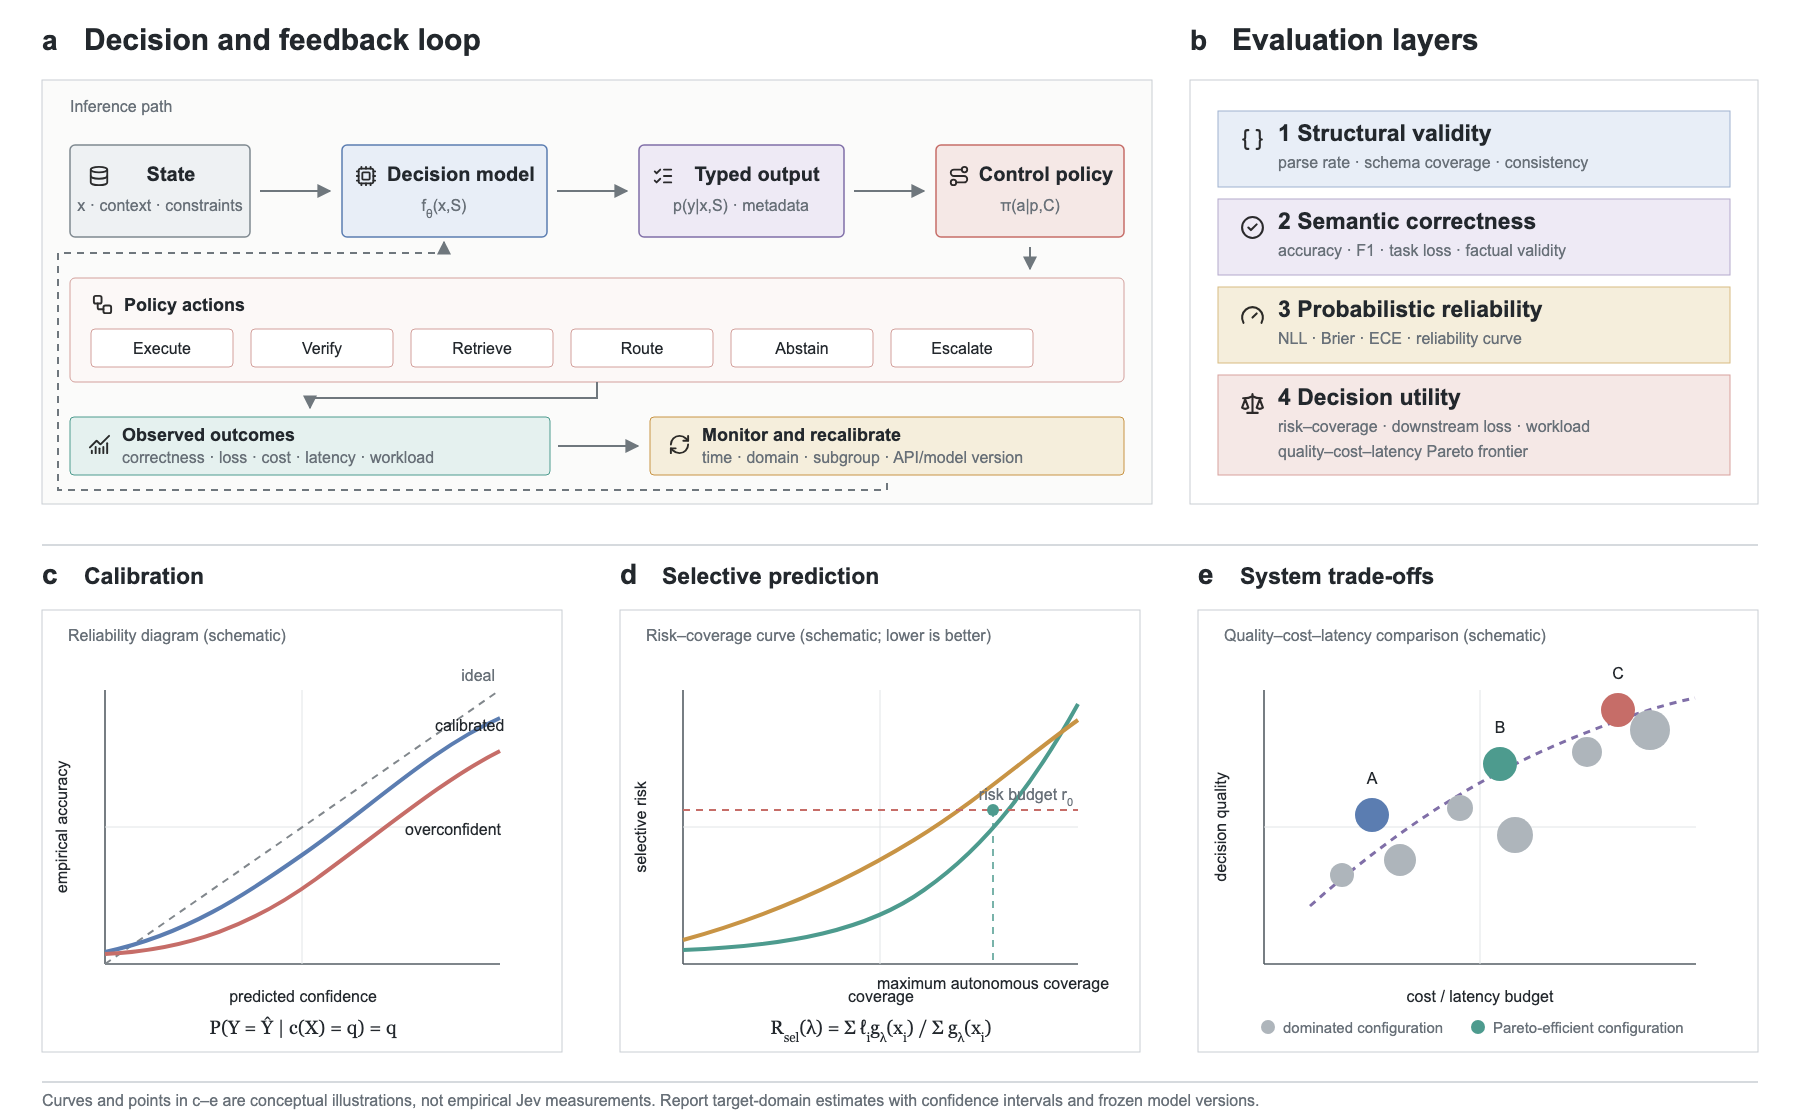
\includegraphics[width=\textwidth]{figures/fig2_evaluation_control_loop.png}
\caption{\textbf{Evaluation framework for machine-native decisions.} \textbf{a}, State, model, typed output, control policy, observed outcomes, and recalibration form a closed loop. \textbf{b}, Four evaluation layers separate structural validity, semantic correctness, probabilistic reliability, and decision utility. \textbf{c--e}, Reliability, risk--coverage, and quality--cost--latency views reveal distinct failure modes. Curves and points are conceptual illustrations and do not report empirical Jev measurements.}
\label{fig:evaluation-loop}
\end{figure*}

\section{Reusable System Patterns}

\paragraph{Smart conditionals.} A model maps unstructured state to a Boolean probability; a cost-sensitive policy executes or escalates. The pattern fits frequent, well-defined, quickly auditable decisions. Concept drift and threshold reuse across businesses are major risks.

\paragraph{Intent and model routing.} A decision model selects a tool, workflow, or downstream model. Router accuracy and final task success should be reported separately, including safety and privacy effects of a wrong route. A 2026 robustness study found category-rigid behavior in preference-based routers and cases where jailbreak prompts were sent to weaker models \cite{kassem2026routerfragility}.

\paragraph{Document triage.} Many typed questions share a contract, ticket, or medical record. Parallel evaluation can reduce latency if cross-question constraints are checked. Low-confidence examples enter a human queue, whose finite capacity determines a feasible threshold.

\paragraph{Agent action gating.} A generative model proposes a plan, a decision model assesses permission or risk, and deterministic code enforces policy. The gate should be calibrated on full agent trajectories because isolated question-answering data miss compounding tool errors.

\paragraph{Retrieval, ranking, and verification.} A decision component can decide whether to retrieve, select evidence, or verify a claim. Label quality depends on corpus freshness. Confidence should target ``safe to act under current evidence,'' a more operational event than timeless factual truth.

\section{Jev as a Contemporary Case Study}

\subsection{Public artifacts}

At the review cutoff, TypeSafe provided product documentation, a confidence guide, an evaluation site, and a Python adapter \cite{typesafe2026docs,typesafe2026confidence,typesafe2026evals,typesafe2026adapter}. The interface centers on state, questions, and Choice/Score/Noul types. The adapter exposes a comparable surface over conventional LLM APIs and enables interface-level baselines. The launch article positions Jev as a System One model and reports RLCD, a parallel sampler, low latency, and low price \cite{almeida2026jev}.

\subsection{Evidence audit}

\begin{table}[t]
\centering\small
\begin{tabular}{p{.18\linewidth}p{.24\linewidth}p{.25\linewidth}p{.24\linewidth}}
\toprule
Claim & Available evidence & Supported interpretation & Needed test \\
\midrule
Typed outputs & Official docs and SDK & API exposes predefined structures & Schema coverage and boundary failures \\
``Zero hallucinations'' & Vendor limits it to schema matching & Format-validity claim & Factual accuracy and harmful actions \\
Calibrated probabilities & Confidence docs and vendor evaluations & Reliability is a design goal & Independent ECE/Brier under shift \\
70--500 ms; USD 0.042/MTok & Launch post & Public performance/price hypothesis & Region, concurrency, length, tail latency \\
RLCD yields calibration & Method name and overview & Reported training direction & Objective, data, ablation, replication \\
Frontier task ability & Vendor evaluation & Self-report under its protocol & Version-frozen third-party blind test \\
\bottomrule
\end{tabular}
\caption{Evidence audit for public Jev claims as of 21 September 2026.}
\label{tab:jev-audit}
\end{table}

Jev's current scientific value lies primarily in its interface proposition: types, probabilities, and multi-question batching become first-class concepts. Whether it constitutes a new model class depends on undisclosed architectural distinctions and reproducible results. If the implementation is a general generator plus a constraint layer, its main contribution resides at the system interface. A representation, objective, and inference procedure designed natively for decisions could establish a distinct speed--quality--calibration frontier.

\subsection{A fair replication protocol}

An independent comparison should include four baseline families: a discriminative encoder, a general LLM with structured output, the same LLM through the public adapter, and Jev's native interface. Tasks should cover Boolean, enumerated, ordinal, multi-question consistency, and open-set abstention. Every system receives the same state and candidate set; prompts and versions are frozen; ground truth comes from independent annotation or executable verification. Primary results should present a quality--cost--latency Pareto surface, reliability diagrams, risk--coverage curves, schema validity, logical conflict rate, and out-of-distribution degradation. When an endpoint cannot be pinned, repeated measurements across dates can quantify version drift.

\section{Open Challenges}

\paragraph{Open-world inputs and closed decisions.} Candidate sets improve control and create out-of-set failures. Systems need an explicit unknown option, open-set detection, or dynamic schemas, while preventing ``other'' from becoming an uninformative escape.

\paragraph{Local calibration.} Confidence depends on domain, prompt, label definition, time, and calling policy. Continuous monitoring, rolling recalibration, and change detection are deployment infrastructure. Marginal guarantees require scrutiny when exchangeability fails.

\paragraph{Parallelism and consistency.} Parallel answers over shared state reduce latency and can ignore dependencies. Factor graphs, logic layers, energy functions, or posterior projection may combine throughput with global constraints.

\paragraph{Labels and delayed utility.} High-value decisions often lack immediate ground truth, and historical human choices contain systematic bias. Offline accuracy may reward imitation of that bias. Causal evaluation, delayed-feedback learning, and multi-expert deferral deserve a place in benchmarks.

\paragraph{Compositional safety.} A calibrated one-step model can accumulate risk inside a looping agent. Evaluation should move from isolated predictions to trajectories, asking whether errors are recoverable, when calls cascade, and whether an attacker can manipulate confidence gates.

\paragraph{Commercial reproducibility.} Endpoint updates, rate limits, and price changes rapidly age conclusions. Versioned datasets, raw logs, containerized evaluators, dated results, and independently hosted blind tests are more durable than a one-off leaderboard.

\section{Research Agenda}

Seven directions are immediately actionable. First, release losses, data recipes, and ablations for calibration-aware decision training. Second, define interoperable semantics for choices, ordinals, sets, abstention, and cost matrices. Third, construct cross-domain and longitudinal calibration suites large enough for subgroup estimates. Fourth, evaluate real action consequences and report Pareto fronts under several cost assumptions. Fifth, study grammar validity, probabilistic coherence, and logical consistency jointly. Sixth, adopt traceable model cards and frozen snapshots for commercial endpoints. Seventh, develop hybrid systems in which generative models propose and explain, decision models select and gate, and formal rules enforce inviolable policy.

\section{Conclusion}

Jev makes a longstanding engineering requirement unusually visible: software needs outputs that are validatable, probabilistically interpretable, and connected to control flow. The scientific basis spans mature but fragmented literatures. Structured output reduces interface failure, calibration gives confidence statistical meaning, selective prediction converts risk into coverage, decision-focused learning links prediction to utility, and routing allocates compute and expertise.

Building on TypeSafe's machine-native intelligence and System One thesis, this survey treats these components as one object of evaluation through an operational definition, a five-dimensional taxonomy, and a four-layer framework. Decisive evidence will require open technical details, cross-domain replication, and workflow-level outcomes. Jev is presently best understood as a testable contemporary case and product signal. The enduring research target is a measurable contract: valid types, reliable probabilities, controlled risk, transparent cost, and a principled handoff when the environment changes.

\bibliographystyle{plain}
\bibliography{references}
\end{document}
